\documentclass[10pt,a4paper]{article}
\usepackage[utf8]{inputenc}
\usepackage{amsmath}
\usepackage{amsfonts}
\usepackage{amssymb}
\usepackage{graphicx}
\usepackage{xcolor}
\usepackage{array}
\usepackage{tcolorbox}
\usepackage{float}
\usepackage{subfig}
\usepackage{parskip}
\usepackage{verbatim}
\usepackage[left=2cm,right=2cm,top=2cm,bottom=2cm]{geometry}
\usepackage{sectsty}
\sectionfont{\usefont{OT1}{phv}{b}{n} \sectionrule{0pt}{0pt}{-5pt}{3pt}}
\author{Songtuan Lin u6162630}
\title{Assignment 1}
\newcolumntype{P}[1]{>{\centering\arraybackslash}p{#1}}
\begin{document}
\maketitle

\section*{Question 1}
For simplicity, I will assume the \textit{HTTP Request} message the server received request a Web Page. 
\begin{figure}[H]
	\center
	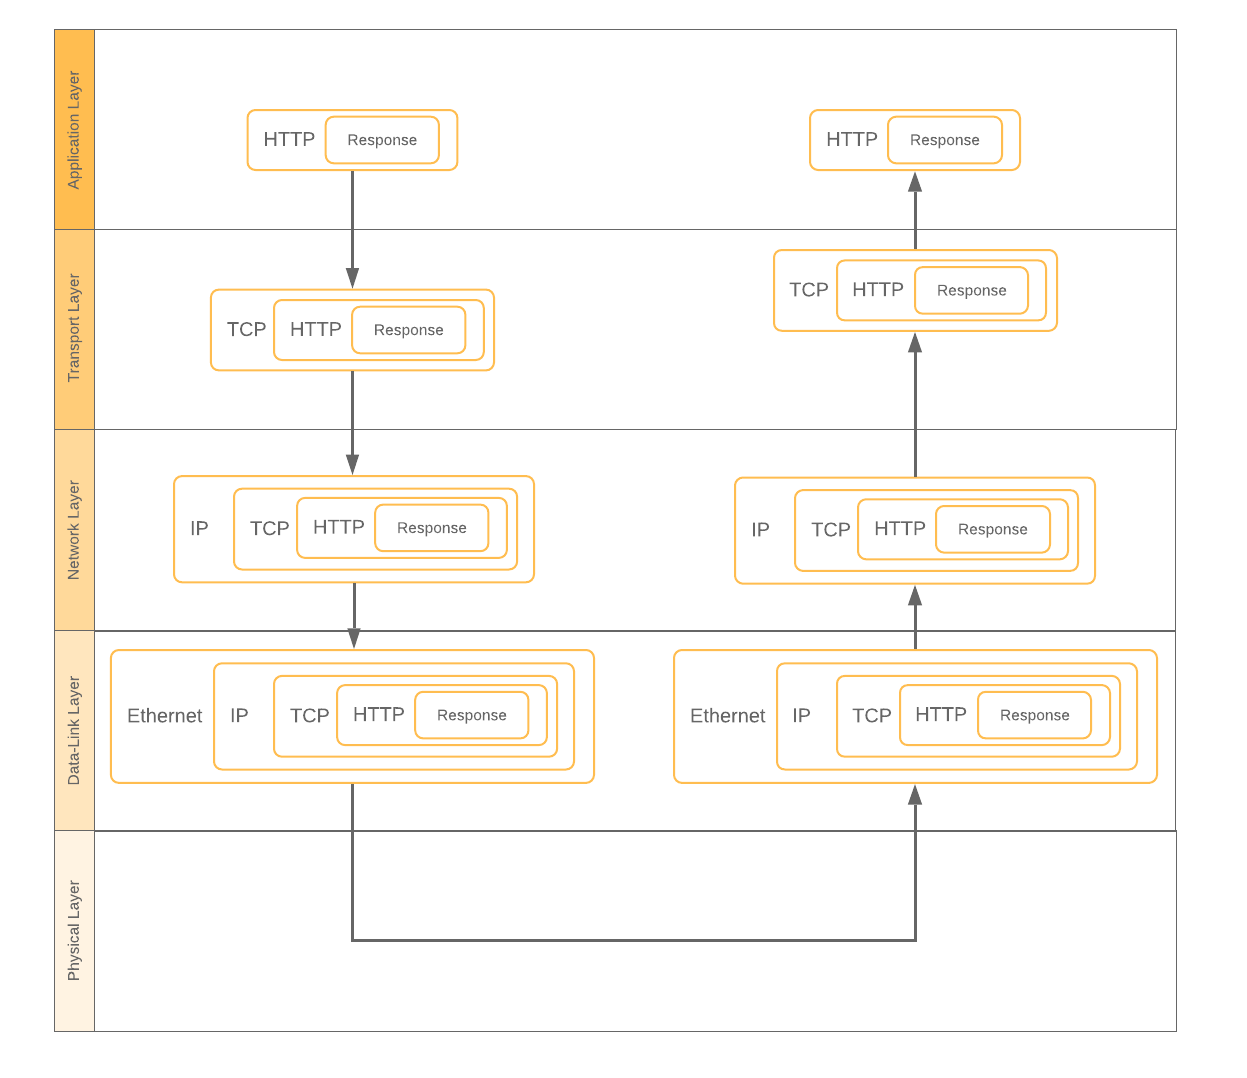
\includegraphics[scale=0.7]{Layers}
	\caption{Transmission through Layers}
	\label{fig_1}
\end{figure}
By comparing Figure \ref{fig_1} with the original Figure, it can be seen that the HTTP Response message will go through the same Network Layer as the HTTP Request message. The only difference shown in these two figures is the \textit{Request} field and \textit{Response} field. Particularity, in this example, the client \textit{request} a Web Page and the server \textit{response} the corresponding html file. Indeed, this simple observation implies a general rule for the communication through computer network:
\begin{center}
	\begin{tcolorbox}[colback=lightgray, width=0.75\textwidth]
		The message delivery within computer network must go through a series of fixed stages and Each stage will accomplish some specific functions to support the delivery.
	\end{tcolorbox}
\end{center}
Technically, each stage correspond to one Layer and form the modern \textit{Layered-Architecture}, as illustrated in Figure \ref{fig_1}. Furthermore, in order to maintain the generality of the message flow within Computer Network, which means the message can be decoded(understood) by different computer in this network, additional rules that specify how each layer accomplish their function have been made. These layer-specific rules are called \textit{protocol}, \textsf{e.g.} HTTP in Application Layer, TCP in Transport Layer, etc. Generally, each protocol need to add some extra information to the original message in order to accomplish their function. This additional information is called \textit{head}. \textsf{e.g.} HTTP head, TCP head, etc. In the following part, I will briefly explain the function and some common protocols corresponding to each layer:
\begin{itemize}
	\item \textbf{Application Layer}: Application Layer produce the message that will be delivered and transfer it to next Transport Layer. Some popular Application Layer protocols include: HTTP, FTP, etc.
	\item \textbf{Transport Layer}: Transport Layer accomplish the preparation tasks before the delivery, e.g. specify the source and target application of the message, maintain the connection between client and server. The common Transport Layer protocols include: TCP and UDP.
	\item \textbf{Network Layer}: Network Layer determine the route of message delivery, which is one of the most important function. The common Network Layer protocols include OSPF, BGP, etc.
	\item \textbf{Data-Link Layer}: Data-Link Layer further determine the route based on the route calculated by Network Layer. The common protocols in Data-Link Layer include Ethernet, WIFI protocol family, etc.
	\item \textbf{Physical Layer}: Physical Layer is responsible for the actual  transmission.  
\end{itemize}
The above explanation may be too abstract. Indeed, we can think Computer Network as a real world package delivery system, hence, we can have a concrete understand about Layer-Architecture by going through an example: Assume a package delivery company have a package that want to be delivered from Australia to China. The entire delivery process, from Computer Network perspective, can be expressed as:
\begin{enumerate}
	\item The Application Layer get a package from customer that need to be delivered.
	\item The Transport Layer confirm this package delivery order.
	\item The Network Layer determine the route of delivery. Particularly, it determine  which country will be in the delivery path, e.g. Australia $\rightarrow$ Indian $\rightarrow$ China
	\item The Data-Link Layer determine the route that how package will be delivered within country.
	\item The physical Layer carry the package and do the actual transmission.
\end{enumerate}
The above discussion give a theory explanation about Layer-Architecture. Indeed, by using software tools like Wireshark and cURL, we can do some practical experiments to see how Layered-Architecture work. These practical experiments will be demonstrated in the rest question within this assignment.

\section*{Question 2}
In this question, I will use cURL to inspect HTTP protocol. This experiment can illustrate the format of HTTP head. In order to complete this question, firstly, I need to configure my web server following the setting up instruction described in this question. Particularly, the web server I used is a droplet from Digital-Ocean with IP address: 188.166.167.192. After I have deployed my web server, I can send a HTTP request through cURL by using following command:
\begin{quote}
	\center
	curl -v http://188.166.167.192:8000
\end{quote} 
The output of this cURL command is shown in Figure \ref{co},
\begin{figure}[ht]
	\center
	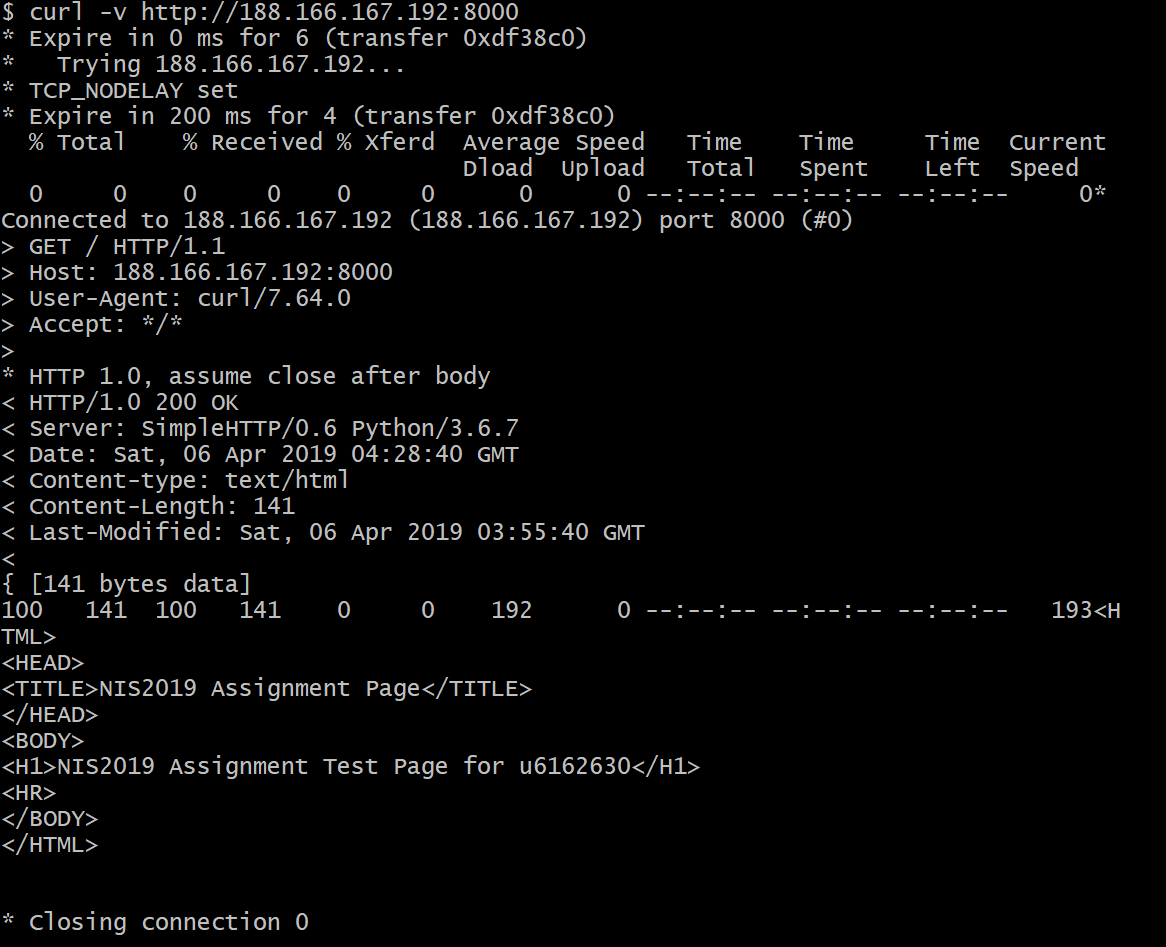
\includegraphics[width = 0.5\textwidth, height = 5cm]{cURL_1}
	\caption{Output of cURL}
	\label{co}
\end{figure}
In which, there are several important content:
\begin{enumerate}
	\item HTTP Request message, which consist the lines start with '$>$'.
	\item HTTP Response message with the HTML file required by client, which consist of the lines start with '$<$'.
\end{enumerate}
By inspecting these two HTTP messages, we can identify that the format of these messages follow the definition in \cite{rfc2616}, which is the standard of HTTP protocol. Even though cURL provide a useful tool to generate HTTP message, the majority of HTTP message in real world is produced by Web Browser. Hence, in Question 3, I will demonstrate how to use HTTP Request to retrieve the same Web Page through Web Browser.

\begin{comment}
\begin{enumerate}
	\item HTTP Request message, which consist of the lines start with '$>$'. Each line, according to \cite{rfc2616}, have the following purpose:
		\begin{itemize}
			\item \textbf{Head Line}: This first line specify the request method and the HTTP protocol version. 
			\item \textbf{Host}: Specify the IP address or domain name of the server. In this example, the IP address of server is: 188.166.167.192.
			\item \textbf{User-Agent}: Specify the application that sent this request message along with its' version. In this example, the request is come from  cURL tool.
			\item \textbf{Accept}: Specify the media types which are acceptable for the client. \textsf{i.e.} video stream and audio.
		\end{itemize}
	\item HTTP Response message, which consist of the lines start with '$<$'. The meaning of each line is:
		\begin{itemize}
			\item \textbf{Head Line}: Serve the same purpose as that in Response message
			\item \textbf{Server}: Specify the server application
			\item \textbf{Date}: The date this response was sent
			\item \textbf{Content-Type}: Specify the file type that this response message will send
			\item \textbf{Content-Length}: Specify the length of the file that will be transformed
			\item \textbf{Last-Modified}: Specify the last date that the file which are willing to be sent is modified.
		\end{itemize}
	\item HTML file, which locate in the last part of the output. This HTML file is the last part of HTTP Response message and correspond to the Web Page requested by clients.
\end{enumerate}
\end{comment}


Instead of using cURL to send HTTP Request, we can use simple Web Browser to retrieve the same Web Page, which will be shown in Question 3.

\section*{Question 3}
The HTML file that been created in web server can be retrieved through web browser by typing the following command:
\begin{quote}
	\center
	http://188.166.167.192:8000
\end{quote}
The result that displayed in web browser is shown in Figure \ref{web}:
\begin{figure}[H]
	\center
	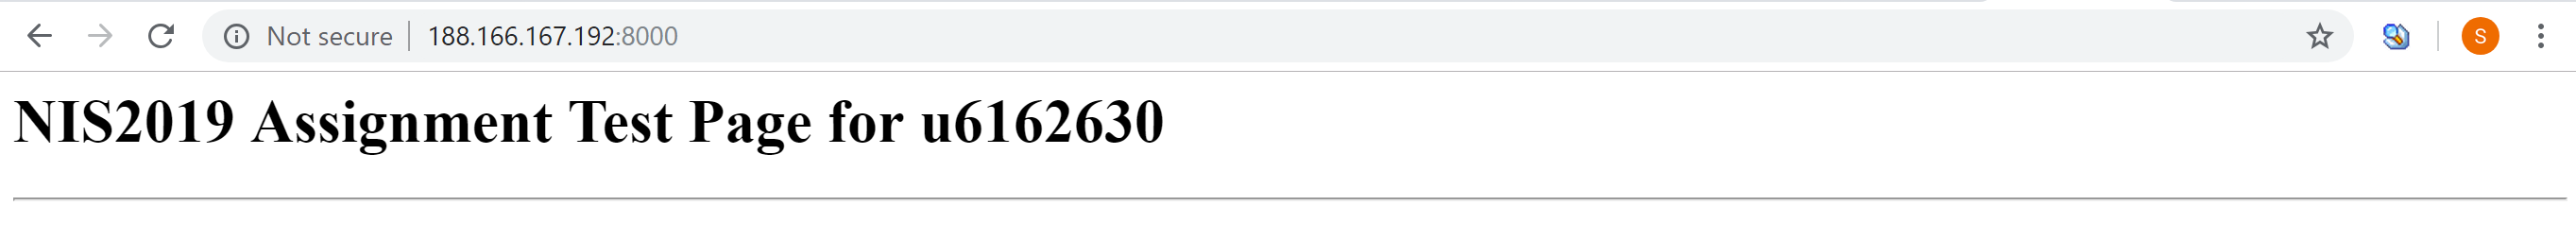
\includegraphics[width = 0.75\textwidth]{web_page}
	\caption{Web Page}
	\label{web}
\end{figure}
In this experiment, the web browser will first send a HTTP Request message to the server. After that, this request message will go through the Layers-Architecture described in Question 1 with the corresponding protocol-head been added, \textsl{i.e.} the TCP head been added in Transport Layer, the IP head been added in Network Layer and the Ethernet head been added in Data-Link Layer. This process can be well illustrated by the Figure 1-4 in Question 1. When the server receive the request, it will reply with a HTTP Response message contain the Web Page required by client. This response message, as indicated in Figure \ref{fig_1}, will go through the same Layers and arrive at the client side. Hence, the web browser can display the Web Page. One more thing that need to be noticed within this process is: When the message arrive at the receiver side, \textsl{e.g.} the server in Figure 1-4 and client in Figure \ref{fig_1}, it will go through the same Layer-Architecture but in inverse order. In the mean time ,each Layer would remove the corresponding protocol head and deliver the message to upper Layer.

\section*{Question 4}
The Question 2 and Question 3 has demonstrated some basic property of HTTP protocol, include its' message format and general delivery process. Indeed, we can also inspect protocols' head other than HTTP by using Wireshark, which is a tool can be used to capture the messages flow within Computer Network. I will demonstrate how to use Wireshark to capture HTTP Request and Response message and use this result to further illustrate Layer-Architecture Model. The following Figure \ref{http_req} and \ref{http_res} are the capture panel of Wireshark, in which, the first two messages are the HTTP message between my computer and the server with IP address 13.211.159.241:
\begin{figure}[H]
	\begin{center}
	\subfloat[Request Message]{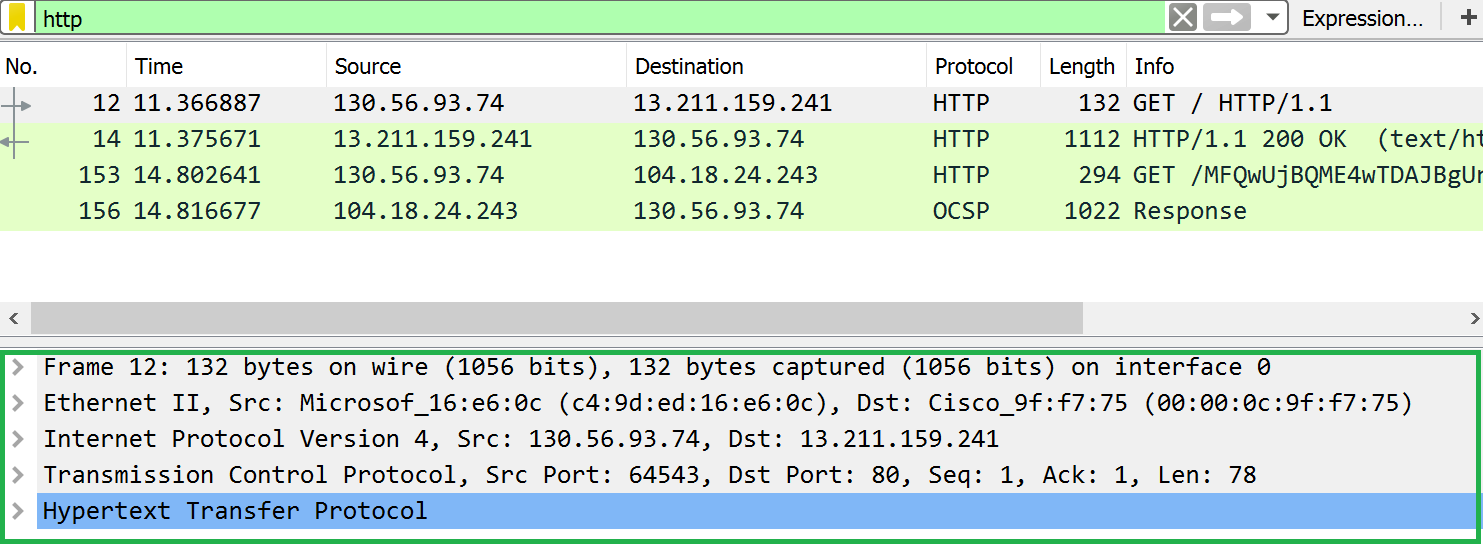
\includegraphics[width=0.45\textwidth, height=3cm]{http_req} \label{http_req}}
	\hspace{1cm}
	\subfloat[Response Message]{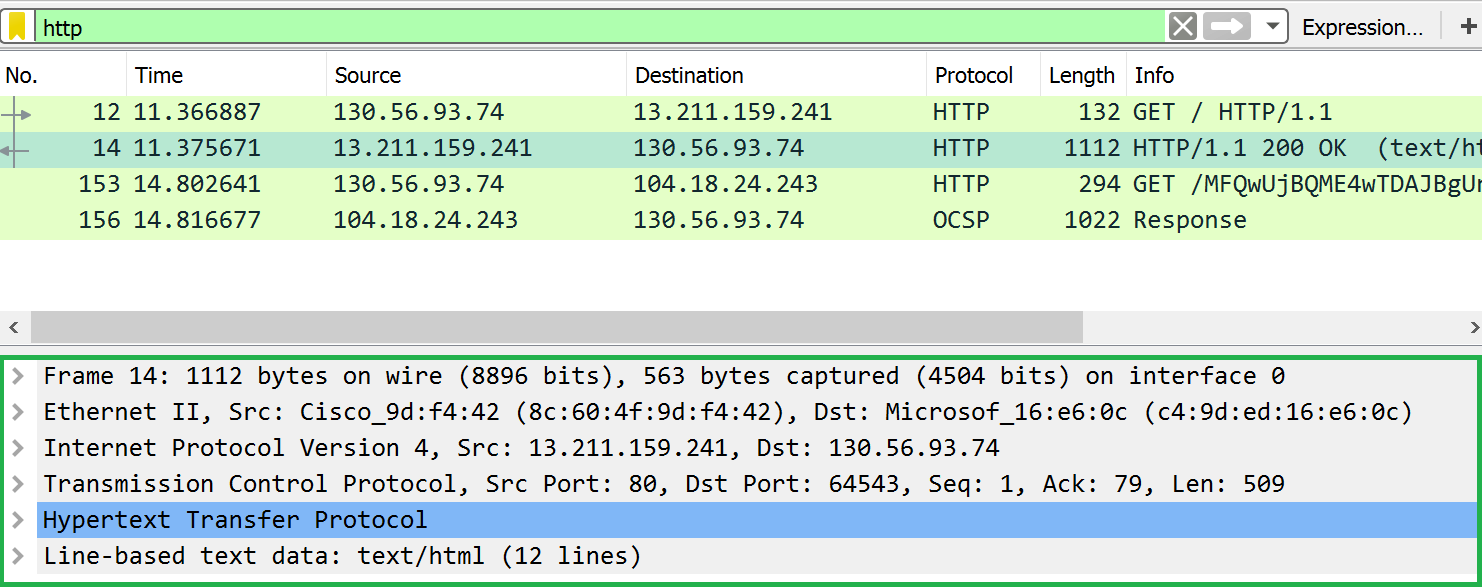
\includegraphics[width=0.45\textwidth, height=3cm]{http_res}\label{http_res}}
	\end{center}
	\caption{Capture Result}
	\label{capture}
\end{figure}
The content of green box within Figure \ref{http_req} and \ref{http_res} illustrate the format of the captured message. Each line within the box corresponding to one protocol head, e.g. The line start with Transmission Control Protocol correspond to TCP head. Particularly, Figure \ref{http_req} indicate the format of HTTP Request message and Figure \ref{http_res} indicate the HTTP Response message. Indeed, these result can be used as a good example to illustrate my discussion of Layer-Architecture in Question 1. I will have a formal discussion of this example in Question 5. In this question, I will use the capture result from Wireshark to inspect some specific fields within protocol head. I will first start with Request message, as illustrated in Figure \ref{http_req_det}:
\begin{figure}[H]
	\center
	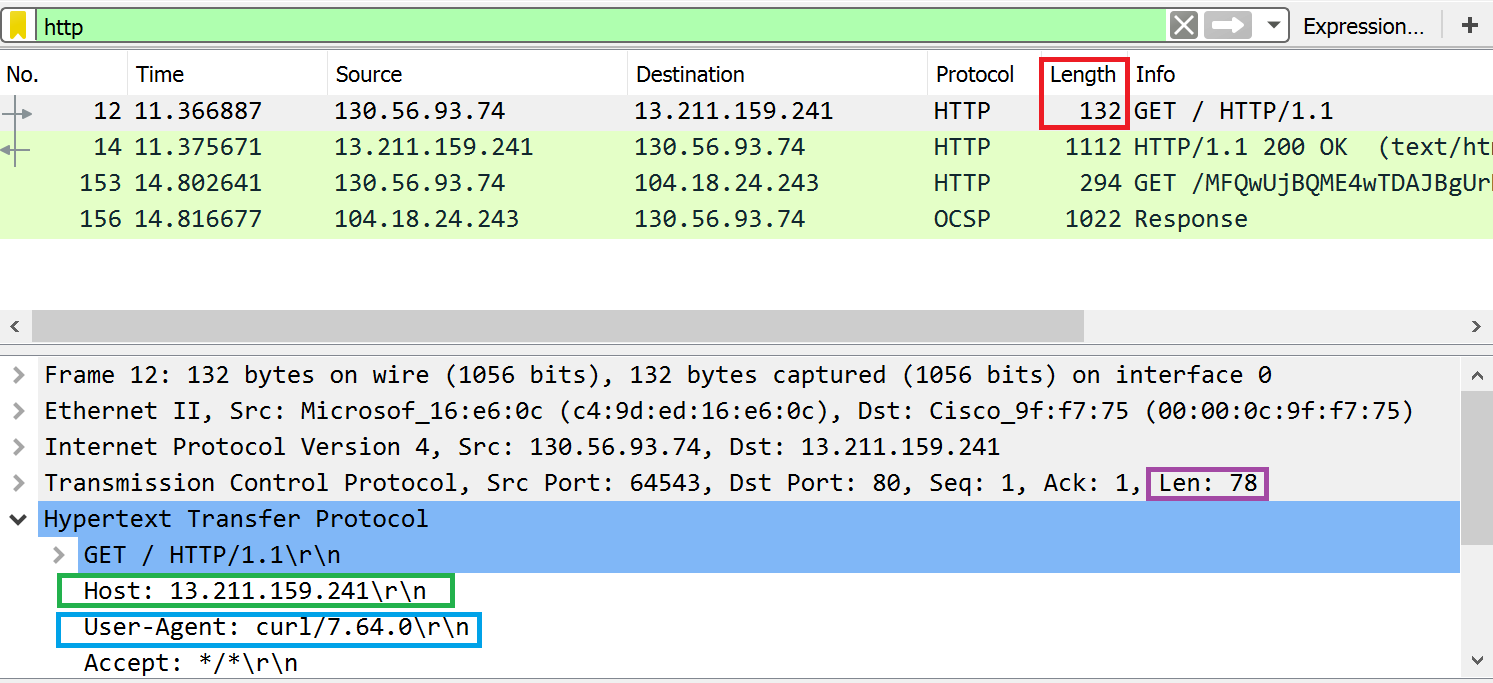
\includegraphics[width = 0.5\textwidth, height = 3cm]{http_req_det}
	\caption{Detail of Request Message}
	\label{http_req_det}
\end{figure}
In which, we can get the following information:
\begin{itemize}
	\item \textbf{The User-Agent Field in HTTP Head}: cURL 7.64.0, which indicate that this request message was sent by application cURL with version 7.64.0 and is shown within the \textbf{blue box}.
	\item \textbf{Host Field in HTTP Head}: 13.211.159.241, which is shown within \textbf{green box}. This IP address is server's IP address.
	\item \textbf{Length of Request Message}: 132 bytes, which is shown within \textbf{red box}. Notice that this length count in all protocol head.
	\item  \textbf{Length of TCP Head}: 78 bytes, which is shown within \textbf{purple box}.
\end{itemize}
After that, we can inspect the detail of Response message as shown in Figure \ref{http_res_det}.
\begin{figure}[H]
	\center
	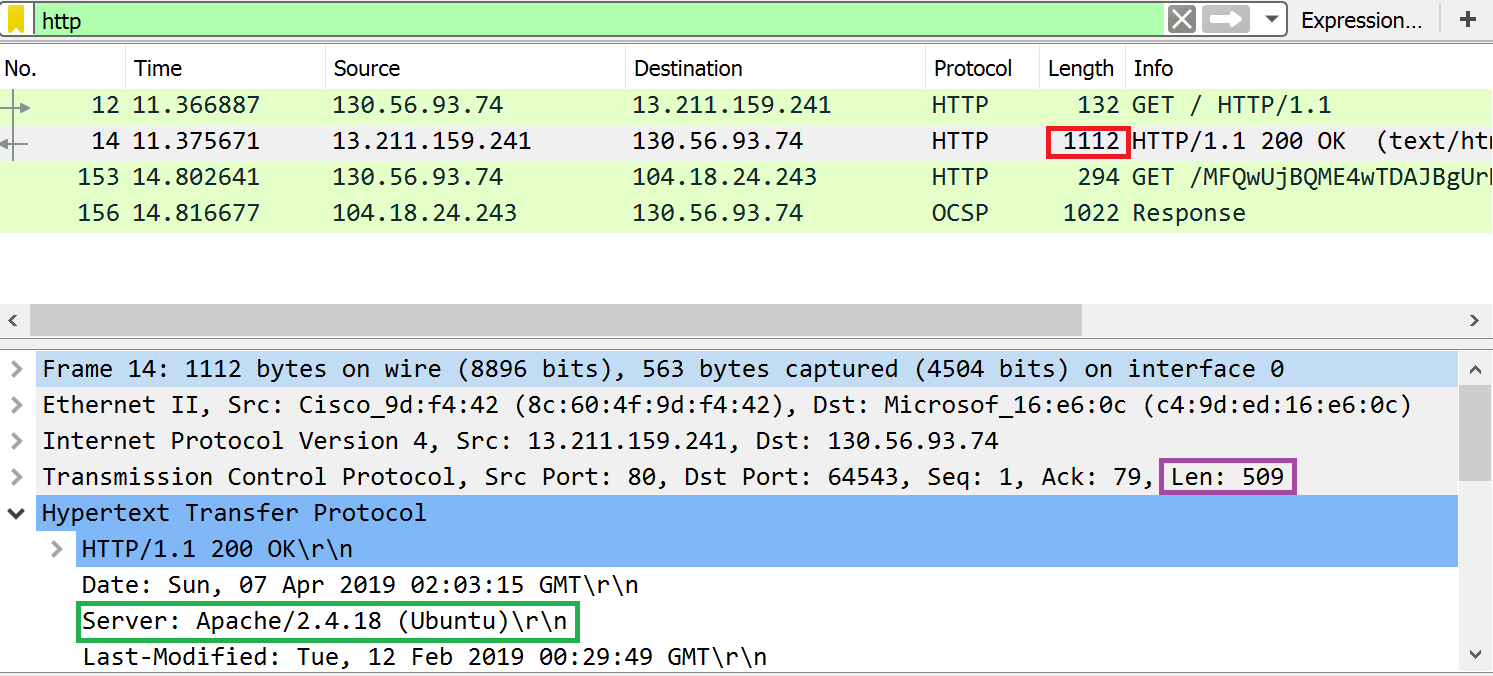
\includegraphics[width = 0.5\textwidth, height = 3cm]{http_res_det}
	\caption{Detail of Response Message}
	\label{http_res_det}
\end{figure}
The following information can be obtained:
\begin{itemize}
	\item \textbf{Server Field in HTTP Head}: Apache/2.4.18, which indicate the response message is given by Apache application with version 2.4.18 and is shown within \textbf{green box}.
	\item \textbf{Length of Response Message}: 1112 bytes, shown within \textbf{red box}.
	\item \textbf{Length of TCP Head}: 509 bytes, shown within \textbf{purple box}.
\end{itemize}

\section*{Question 5}
In Question 1, I have mentioned that each layer in Layer-Architecture will add a specific head to original message. Technical, this process is called encapsulation. In more specific:
\begin{center}
	\begin{tcolorbox}[colback = lightgray, width = 0.75\textwidth]
		\color{black}{\textbf{Encapsulation} is the process that add a protocol-specific head to original message and produce a new one.}
	\end{tcolorbox}
\end{center}
The Wireshark capture result from Question 4 provide us a concrete example that illustrate how encapsulation work. It can be seen from the capture result that in Transport Layer, it add a TCP head to the HTTP packet from Application Layer and produce a \textit{Transport Layer segment}, which means, Transport Layer \textit{encapsulate} HTTP packet into Transport Layer segment with a TCP head. This encapsulation can be demonstrated as:
\begin{equation*}
	\overbrace{\boxed{\text{TCP head}} + \underbrace{\boxed{\text{HTTP head}}}_{\text{HTTP packet}}}^{\text{Transport Layer segment}}
\end{equation*}
Furthermore, the Transport Layer segment will be sent to Network Layer and be encapsulated into \textit{Network Layer packet} with IP head. The encapsulation repeat until the message reach the Physical Layer. In the meantime, final message has the format:
\begin{center}
	\begin{tabular}{|c|c|c|c|}
		\hline
		Ethernet head & IP head & TCP head & HTTP head\\
		\hline
	\end{tabular}
\end{center}
The advantages of using encapsulation is that it separate the function of different Layer, which make the Layer-Architecture easier to maintain and develop. 

By the end of this assignment, I have draw a big picture of Computer Network by giving a general description of Layer-Architecture and use some concrete example to illustrate some important concepts like encapsulation, which is the core part of Layer-Architecture. Additionally, the format of some specific protocol head also be inspected by using tools like Wireshark and cURL.

\bibliography{rfc}
\bibliographystyle{apalike}
\end{document}